\documentclass[]{article}
\usepackage{lmodern}
\usepackage{amssymb,amsmath}
\usepackage{ifxetex,ifluatex}
\usepackage{bm}
\usepackage{soul}
\usepackage[color=yellow]{todonotes}
\usepackage{fixltx2e} % provides \textsubscript
\ifnum 0\ifxetex 1\fi\ifluatex 1\fi=0 % if pdftex
  \usepackage[T1]{fontenc}
  \usepackage[utf8]{inputenc}
\else % if luatex or xelatex
  \ifxetex
    \usepackage{mathspec}
  \else
    \usepackage{fontspec}
  \fi
  \defaultfontfeatures{Ligatures=TeX,Scale=MatchLowercase}
\fi
% use upquote if available, for straight quotes in verbatim environments
\IfFileExists{upquote.sty}{\usepackage{upquote}}{}
% use microtype if available
\IfFileExists{microtype.sty}{%
\usepackage{microtype}
\UseMicrotypeSet[protrusion]{basicmath} % disable protrusion for tt fonts
}{}
\usepackage[margin=1in]{geometry}
\usepackage{hyperref}
\hypersetup{unicode=true,
            pdftitle={7 Introduction to time series analysis in the frequency domain},
            pdfauthor={Edward Ionides},
            pdfborder={0 0 0},
            breaklinks=true}
\urlstyle{same}  % don't use monospace font for urls
\usepackage{color}
\usepackage{fancyvrb}
\newcommand{\VerbBar}{|}
\newcommand{\VERB}{\Verb[commandchars=\\\{\}]}
\DefineVerbatimEnvironment{Highlighting}{Verbatim}{commandchars=\\\{\}}
% Add ',fontsize=\small' for more characters per line
\usepackage{framed}
\definecolor{shadecolor}{RGB}{248,248,248}
\newenvironment{Shaded}{\begin{snugshade}}{\end{snugshade}}
\newcommand{\KeywordTok}[1]{\textcolor[rgb]{0.13,0.29,0.53}{\textbf{#1}}}
\newcommand{\DataTypeTok}[1]{\textcolor[rgb]{0.13,0.29,0.53}{#1}}
\newcommand{\DecValTok}[1]{\textcolor[rgb]{0.00,0.00,0.81}{#1}}
\newcommand{\BaseNTok}[1]{\textcolor[rgb]{0.00,0.00,0.81}{#1}}
\newcommand{\FloatTok}[1]{\textcolor[rgb]{0.00,0.00,0.81}{#1}}
\newcommand{\ConstantTok}[1]{\textcolor[rgb]{0.00,0.00,0.00}{#1}}
\newcommand{\CharTok}[1]{\textcolor[rgb]{0.31,0.60,0.02}{#1}}
\newcommand{\SpecialCharTok}[1]{\textcolor[rgb]{0.00,0.00,0.00}{#1}}
\newcommand{\StringTok}[1]{\textcolor[rgb]{0.31,0.60,0.02}{#1}}
\newcommand{\VerbatimStringTok}[1]{\textcolor[rgb]{0.31,0.60,0.02}{#1}}
\newcommand{\SpecialStringTok}[1]{\textcolor[rgb]{0.31,0.60,0.02}{#1}}
\newcommand{\ImportTok}[1]{#1}
\newcommand{\CommentTok}[1]{\textcolor[rgb]{0.56,0.35,0.01}{\textit{#1}}}
\newcommand{\DocumentationTok}[1]{\textcolor[rgb]{0.56,0.35,0.01}{\textbf{\textit{#1}}}}
\newcommand{\AnnotationTok}[1]{\textcolor[rgb]{0.56,0.35,0.01}{\textbf{\textit{#1}}}}
\newcommand{\CommentVarTok}[1]{\textcolor[rgb]{0.56,0.35,0.01}{\textbf{\textit{#1}}}}
\newcommand{\OtherTok}[1]{\textcolor[rgb]{0.56,0.35,0.01}{#1}}
\newcommand{\FunctionTok}[1]{\textcolor[rgb]{0.00,0.00,0.00}{#1}}
\newcommand{\VariableTok}[1]{\textcolor[rgb]{0.00,0.00,0.00}{#1}}
\newcommand{\ControlFlowTok}[1]{\textcolor[rgb]{0.13,0.29,0.53}{\textbf{#1}}}
\newcommand{\OperatorTok}[1]{\textcolor[rgb]{0.81,0.36,0.00}{\textbf{#1}}}
\newcommand{\BuiltInTok}[1]{#1}
\newcommand{\ExtensionTok}[1]{#1}
\newcommand{\PreprocessorTok}[1]{\textcolor[rgb]{0.56,0.35,0.01}{\textit{#1}}}
\newcommand{\AttributeTok}[1]{\textcolor[rgb]{0.77,0.63,0.00}{#1}}
\newcommand{\RegionMarkerTok}[1]{#1}
\newcommand{\InformationTok}[1]{\textcolor[rgb]{0.56,0.35,0.01}{\textbf{\textit{#1}}}}
\newcommand{\WarningTok}[1]{\textcolor[rgb]{0.56,0.35,0.01}{\textbf{\textit{#1}}}}
\newcommand{\AlertTok}[1]{\textcolor[rgb]{0.94,0.16,0.16}{#1}}
\newcommand{\ErrorTok}[1]{\textcolor[rgb]{0.64,0.00,0.00}{\textbf{#1}}}
\newcommand{\NormalTok}[1]{#1}
\usepackage{longtable,booktabs}
\usepackage{graphicx,grffile}
\makeatletter
\def\maxwidth{\ifdim\Gin@nat@width>\linewidth\linewidth\else\Gin@nat@width\fi}
\def\maxheight{\ifdim\Gin@nat@height>\textheight\textheight\else\Gin@nat@height\fi}
\makeatother
% Scale images if necessary, so that they will not overflow the page
% margins by default, and it is still possible to overwrite the defaults
% using explicit options in \includegraphics[width, height, ...]{}
\setkeys{Gin}{width=\maxwidth,height=\maxheight,keepaspectratio}
\IfFileExists{parskip.sty}{%
\usepackage{parskip}
}{% else
\setlength{\parindent}{0pt}
\setlength{\parskip}{6pt plus 2pt minus 1pt}
}
\setlength{\emergencystretch}{3em}  % prevent overfull lines
\providecommand{\tightlist}{%
  \setlength{\itemsep}{0pt}\setlength{\parskip}{0pt}}
%\setcounter{secnumdepth}{0}
\setcounter{section}{7}
% Redefines (sub)paragraphs to behave more like sections
\ifx\paragraph\undefined\else
\let\oldparagraph\paragraph
\renewcommand{\paragraph}[1]{\oldparagraph{#1}\mbox{}}
\fi
\ifx\subparagraph\undefined\else
\let\oldsubparagraph\subparagraph
\renewcommand{\subparagraph}[1]{\oldsubparagraph{#1}\mbox{}}
\fi

%%% Use protect on footnotes to avoid problems with footnotes in titles
\let\rmarkdownfootnote\footnote%
\def\footnote{\protect\rmarkdownfootnote}

%%% Change title format to be more compact
\usepackage{titling}

% Create subtitle command for use in maketitle
\newcommand{\subtitle}[1]{
  \posttitle{
    \begin{center}\large#1\end{center}
    }
}

\setlength{\droptitle}{-2em}
  \title{7. Introduction to time series analysis in the frequency domain}
  \pretitle{\vspace{\droptitle}\centering\huge}
  \posttitle{\par}
  \author{Edward Ionides}
  \preauthor{\centering\large\emph}
  \postauthor{\par}
  \predate{\centering\large\emph}
  \postdate{\par}
  \date{2/7/2018}


\begin{document}
\maketitle

{
\setcounter{tocdepth}{2}
\tableofcontents
}
\newcommand\prob{\mathbb{P}}
\newcommand\E{\mathbb{E}}
\newcommand\var{\mathrm{Var}}
\newcommand\cov{\mathrm{Cov}}
\newcommand\loglik{\ell}
\newcommand\R{\mathbb{R}}
\newcommand\data[1]{#1^*}
\newcommand\params{\, ; \,}
\newcommand\eqspace{\quad\quad\quad}
\newcommand\lik{\mathscr{L}}
\newcommand\profileloglik[1]{\ell^\mathrm{profile}_#1}
\newcommand\ar{\phi}
\newcommand\ma{\psi}
\newcommand\AR{\Phi}
\newcommand\MA{\Psi}
\newcommand\ev{u}





\begin{center}\rule{0.5\linewidth}{\linethickness}\end{center}

\begin{center}\rule{0.5\linewidth}{\linethickness}\end{center}

Objectives

\begin{itemize}
\tightlist
\item
  This course emphasizes time domain analysis of time series, but we
  also want to be able to present and interpret the frequency domain
  properties of our time series models and data.
\end{itemize}

\begin{enumerate}
\def\labelenumi{\arabic{enumi}.}
\item
  Looking at the frequency components present in our data can help to
  identify appropriate models.
\item
  Looking at the frequency components present in our models can help to
  assess whether they are doing a good job of describing our data.
\end{enumerate}

\begin{center}\rule{0.5\linewidth}{\linethickness}\end{center}

\begin{center}\rule{0.5\linewidth}{\linethickness}\end{center}

\subsection{What is the spectrum of a time series
model?}\label{what-is-the-spectrum-of-a-time-series-model}

\begin{itemize}
\item
  We're going to start by reviewing eigenvectors and eigenvalues of
  covariance matrices. This eigen decomposition also arises elsewhere in
  Statistics, such as the principle component analysis technique in
  multivariate analysis.
\item
  A univariate time series model is a vector-valued random variable
  \(Y_{1:N}\) which we suppose has a covariance matrix \(V\) which is an
  \(N\times N\) matrix with entries \(V_{mn}=\cov(Y_m,Y_n)\).
\item
  \(V\) is a non-negative definite symmetric matrix, and
  \href{https://en.wikipedia.org/wiki/Eigendecomposition_of_a_matrix\#Real_symmetric_matrices}{therefore}
  has \(N\) non-negative eigenvalues \(\lambda_1,\dots,\lambda_N\) with
  corresponding eigenvectors \(\ev_1,\dots,\ev_N\) such that
  \[ V \ev_n = \lambda_n \ev_n.\]
\item
  A basic property of these eigenvectors is that they are orthogonal,
  i.e., \[ \ev_m^T \ev_n = 0 \mbox{ if $m\neq n$}.\]
\item
  We may work with \textbf{normalized} eigenvectors that are scaled such
  that \(\ev_n^T \ev_n = 1\).
\item
  We can also check that the components of \(Y\) in the directions of
  different eigenvectors are uncorrelated. Since
  \(\cov(AY,BY)=A\cov(Y,Y)B^T\), we have

  \begin{eqnarray}
  \cov(\ev_m^T Y, \ev_n^T Y) &= \ev_m^T \cov(Y,Y) \ev_n
  \\
  &= \ev_m^T V \ev_n
  \\
  &=\lambda_n \ev_m^T \ev_n 
  &= \left\{\begin{array}{ll} 
  \lambda_n & \mbox{if $m=n$} \\ 0 & \mbox{if $m\neq n$}
  \end{array}\right.
  \end{eqnarray}

  For the last equality, we have supposed that the eigenvectors are
  normalized.
\item
  Thus, if we knew \(V\), we could convert the model to a representation
  where the observable random variables are uncorrelated.
\item
  Specifically, we could transform the data into its components in the
  directions of the eigenvectors of the model. An uncorrelated (or, in
  the Gaussian case, independent) model would then become appropriate
  for this transformation of the data.
\item
  Let's see how to do that for a stationary time series model, say 100
  observations from an AR(1) model with autoregressive coefficient 0.8.
\end{itemize}

\begin{Shaded}
\begin{Highlighting}[]
\NormalTok{N <-}\StringTok{ }\DecValTok{100}
\NormalTok{phi <-}\StringTok{ }\FloatTok{0.8}
\NormalTok{sigma <-}\StringTok{ }\DecValTok{1}
\NormalTok{V <-}\StringTok{ }\KeywordTok{matrix}\NormalTok{(}\OtherTok{NA}\NormalTok{,N,N)}
\ControlFlowTok{for}\NormalTok{(m }\ControlFlowTok{in} \DecValTok{1}\OperatorTok{:}\NormalTok{N) }\ControlFlowTok{for}\NormalTok{(n }\ControlFlowTok{in} \DecValTok{1}\OperatorTok{:}\NormalTok{N) V[m,n] <-}\StringTok{ }\NormalTok{sigma}\OperatorTok{^}\DecValTok{2} \OperatorTok{*}\StringTok{ }\NormalTok{phi}\OperatorTok{^}\KeywordTok{abs}\NormalTok{(m}\OperatorTok{-}\NormalTok{n) }\OperatorTok{/}\StringTok{ }\NormalTok{(}\DecValTok{1}\OperatorTok{-}\NormalTok{phi}\OperatorTok{^}\DecValTok{2}\NormalTok{)}
\NormalTok{V_eigen <-}\StringTok{ }\KeywordTok{eigen}\NormalTok{(V,}\DataTypeTok{symmetric=}\OtherTok{TRUE}\NormalTok{)}
\NormalTok{oldpars <-}\StringTok{ }\KeywordTok{par}\NormalTok{(}\DataTypeTok{mfrow=}\KeywordTok{c}\NormalTok{(}\DecValTok{1}\NormalTok{,}\DecValTok{2}\NormalTok{))}
\KeywordTok{matplot}\NormalTok{(V_eigen}\OperatorTok{$}\NormalTok{vectors[,}\DecValTok{1}\OperatorTok{:}\DecValTok{5}\NormalTok{],}\DataTypeTok{type=}\StringTok{"l"}\NormalTok{)}
\KeywordTok{matplot}\NormalTok{(V_eigen}\OperatorTok{$}\NormalTok{vectors[,}\DecValTok{6}\OperatorTok{:}\DecValTok{9}\NormalTok{],}\DataTypeTok{type=}\StringTok{"l"}\NormalTok{)}
\end{Highlighting}
\end{Shaded}

\begin{center}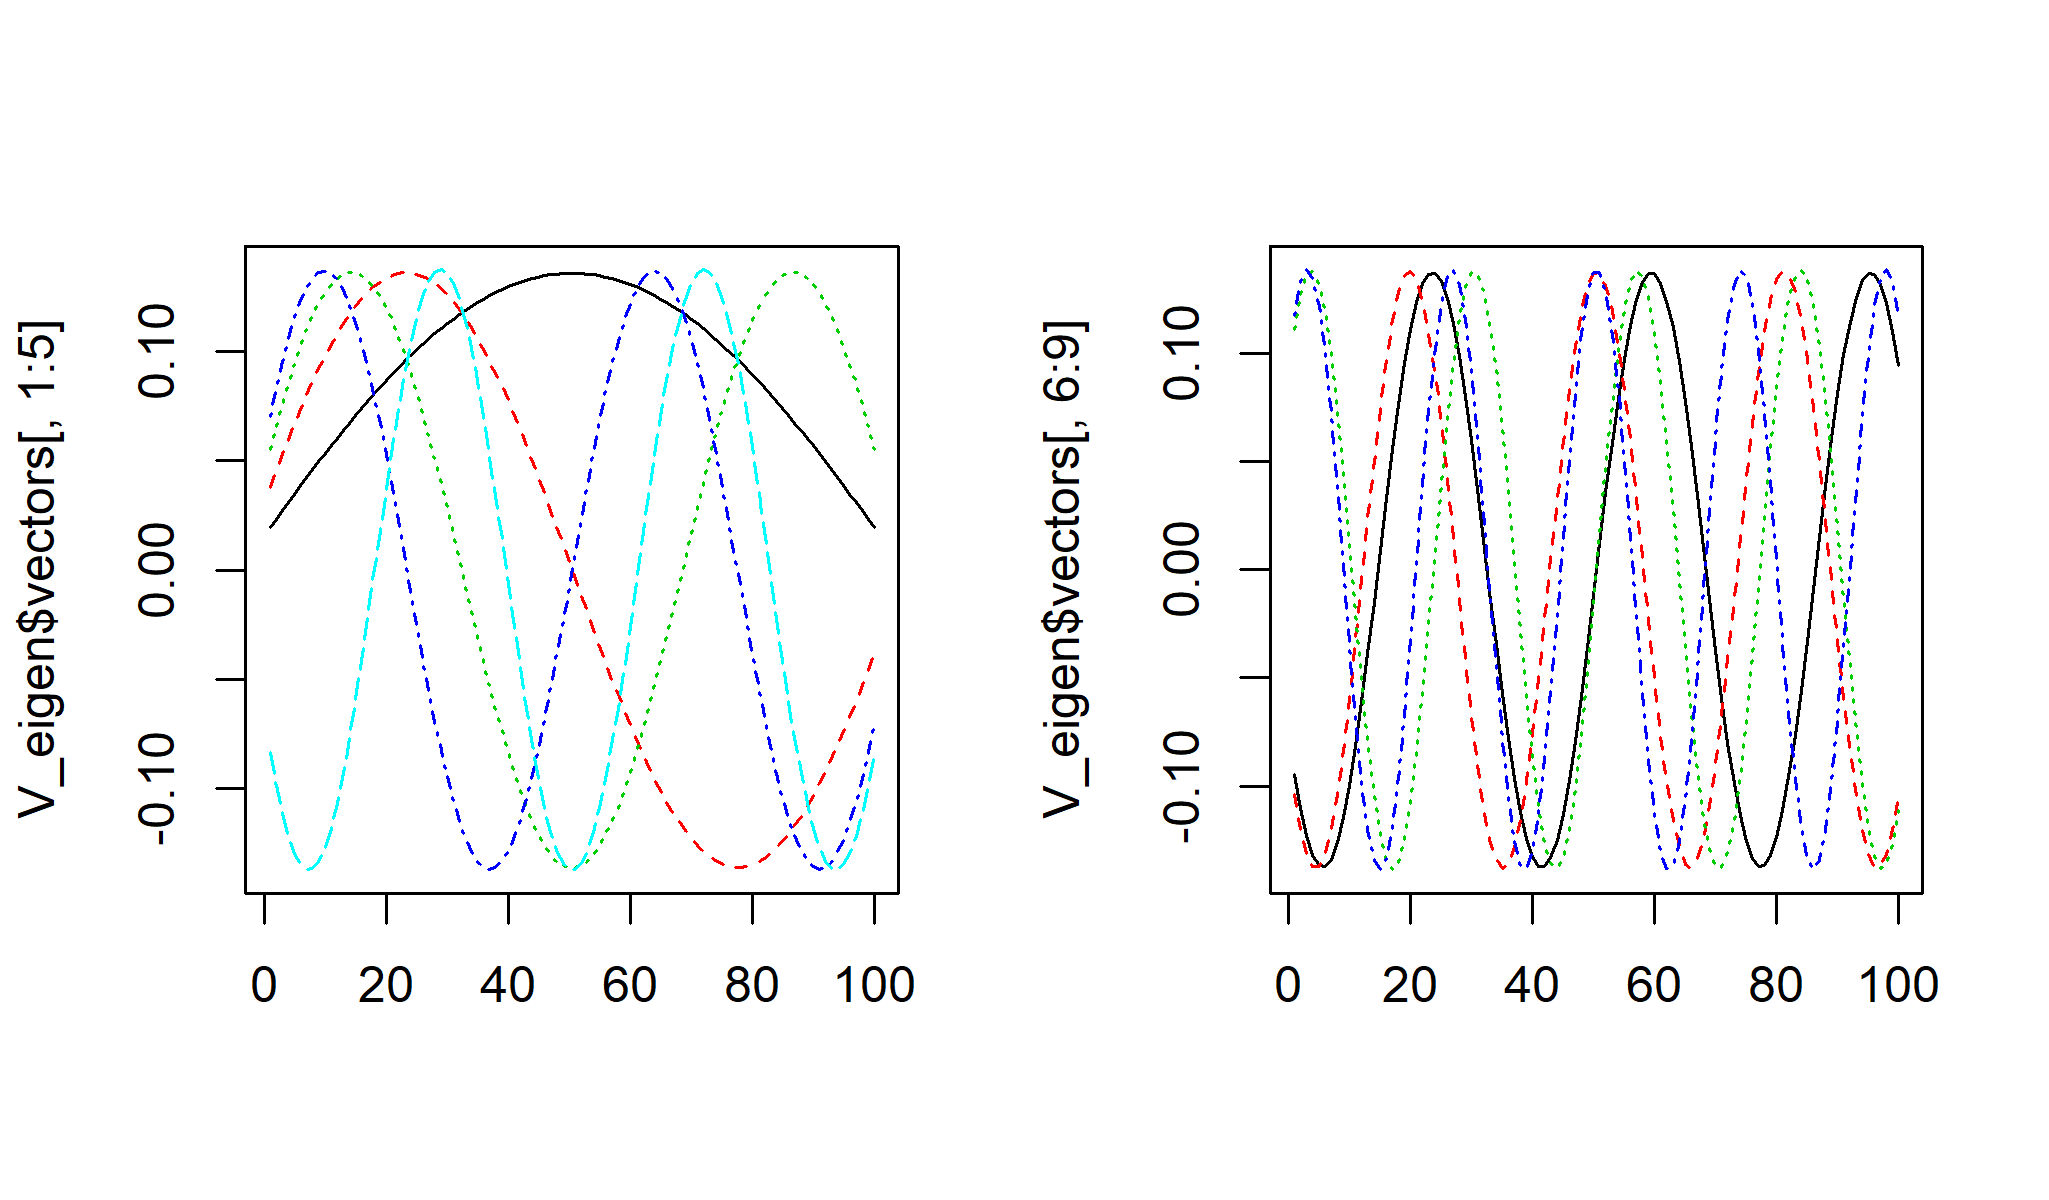
\includegraphics{figure/intro-eigen-1} \end{center}

\begin{Shaded}
\begin{Highlighting}[]
\KeywordTok{par}\NormalTok{(oldpars)}
\end{Highlighting}
\end{Shaded}

\begin{itemize}
\item
  We see that the eigenvectors, plotted as functions of time, look like
  sine wave oscillations.
\item
  The eigenvalues are
\end{itemize}

\begin{Shaded}
\begin{Highlighting}[]
\KeywordTok{round}\NormalTok{(V_eigen}\OperatorTok{\$}\NormalTok{values[}\DecValTok{1}\OperatorTok{:}\DecValTok{9}\NormalTok{],}\DecValTok{2}\NormalTok{)}
\end{Highlighting}
\end{Shaded}

\begin{verbatim}
## [1] 24.59 23.44 21.73 19.70 17.57 15.51 13.61 11.91 10.42
\end{verbatim}

\begin{itemize}
\item
  We see that the eigenvalues are decreasing. For this model, the
  components of \(Y_{1:N}\) with highest variance correspond to
  long-period oscillations.
\item
  Are the sinusoidal eigenvectors a special feature of this particular
  time series model, or something more general?
\end{itemize}

\begin{center}\rule{0.5\linewidth}{\linethickness}\end{center}

\begin{center}\rule{0.5\linewidth}{\linethickness}\end{center}

\subsubsection{The eigenvectors for a long stationary time series
model}\label{the-eigenvectors-for-a-long-stationary-time-series-model}

\begin{itemize}
\item
  Suppose \(\{Y_n,-\infty<n<\infty\}\) has a stationary autocovariance
  function \(\gamma_h\).
\item
  We write \(\Gamma\) for the infinite matrix with entries
  \[ \Gamma_{m,n} = \gamma_{m-n} \quad \mbox{for all integers $m$ and $n$}.\]
\item
  An infinite eigenvector is a sequence
  \(\ev=\{\ev_n, -\infty<n<\infty\}\) with corresponding eigenvalue
  \(\lambda\) such that \[\Gamma \ev = \lambda \ev,\] or, writing out
  the matrix multiplication explicitly,
  \[\sum_{n=-\infty}^\infty \Gamma_{m,n} \ev_n = \lambda \ev_m\quad \mbox{for all $m$}.\]
\item
  Now, let's look for a sinusoidal solution, \(\ev_n = e^{i\omega n}\).
  Then,

  \begin{eqnarray}
  \sum_{n=-\infty}^\infty \Gamma_{m,n} \ev_n 
  &=& \sum_{n=-\infty}^\infty \gamma_{m-n} \ev_n 
  \\
  &=& \sum_{h=-\infty}^\infty \gamma_{h}  \ev_{m-h} \quad \mbox{setting $h=m-n$}
  \\
  &=& \sum_{h=-\infty}^\infty \gamma_{h}  e^{i\omega(m-h)}
  \\
  &=& e^{i\omega m} \sum_{h=-\infty}^\infty \gamma_{h}  e^{-i\omega h}
  \\
  &=& \ev_m \lambda \mbox{ for } \lambda= \sum_{h=-\infty}^\infty \gamma_{h}  e^{-i\omega h}
  \end{eqnarray}
\item
  This calculation shows that \[\ev_n(\omega) = e^{i\omega n}\] is an
  eigenvector for \(\Gamma\) for any choice of \(\omega\). The
  corresponding \hl{eigenvalue function},
  \[\lambda(\omega)= \sum_{h=-\infty}^\infty \gamma_{h}  e^{-i\omega h},\]
  is called the \hl{\textbf{spectral density function}. It is calculated as
  the \textbf{Fourier transform} of $\gamma_h$ at \emph{frequency}
  $\omega$.}
\item
  It was convenient to do this calculation with complex exponentials.
  However, writing
  \[ e^{i\omega n} = \cos(\omega n) + i \sin(\omega n)\] we see that the
  real and imaginary parts of this calculation in fact give us two real
  eigenvectors, \(\cos(\omega n)\) and \(\sin(\omega n)\).
\item
  Assuming that this computation for an infinite sum represents a limit
  of increasing dimension for finite matrices, we have found that the
  eigenfunctions for any long, stationary time series model are
  approximately sinusoidal.
\item
  \hl{For the finite time series situation, we only expect $N$
  eigenvectors for a time series of length $N$}. We have one
  eigenvector for \(\omega=0\), two eigenvectors corresponding to sine
  and cosine functions with frequency
  \[\omega_{n} = 2\pi n/N, \mbox{ for $0<n<N/2$},\] and, if \(N\) is
  even, a final eigenvector with \hl{frequency} \[\omega_{(N/2)} = \pi.\]
\item
  These sine and cosine vectors are called the \textbf{Fourier basis}.
\end{itemize}

\subsection{Frequency components of the data and their representation
via the Fourier
transform}\label{frequency-components-of-the-data-and-their-representation-via-the-fourier-transform}

\begin{itemize}
\item
  The \hl{\textbf{frequency components} of $Y_{1:N}$} are the components in
  the directions of these eigenvectors. Equivalently, we could say \hl{they
  are the representation of $Y_{1:N}$ in the Fourier basis.}
  Specifically, we write

  \begin{eqnarray}
  C_n &=& \frac{1}{\sqrt{N}}\sum_{k=1}^N Y_k\cos(\omega_n k) \mbox{ for $0\le n\le N/2$},
  \\
  S_n &=& \frac{1}{\sqrt{N}}\sum_{k=1}^N Y_k\sin(\omega_n k) \mbox{ for $1\le n\le N/2$}.
  \end{eqnarray}
\item
  Similarly, the \textbf{frequency components} of data
  \(\data{y_{1:N}}\) are

  \begin{eqnarray}
  \data{c_n} &=& \frac{1}{\sqrt{N}}\sum_{k=1}^N \data{y_k}\cos(\omega_n k) \mbox{ for $0\le n\le N/2$},
  \\
  \data{s_n} &=& \frac{1}{\sqrt{N}}\sum_{k=1}^N \data{y_k}\sin(\omega_n k) \mbox{ for $1\le n\le N/2$}.
  \end{eqnarray}
\item
  The frequency components of the data are often written as real and
  imaginary parts of the \textbf{discrete Fourier transform},

  \begin{eqnarray}
  \data{d_n} &=& \frac{1}{\sqrt{N}} \sum_{k=1}^N \data{y_k} e^{2\pi i n/N}
  \\
  &=&\data{c_n} + i\data{s_n}
  \end{eqnarray}
\item
  Here, we have made a decision to introduce a normalizing constant of
  \(1/\sqrt{N}\). There are various choices about signs and factors of
  \(2\pi\), \(\sqrt{2\pi}\) and \(\sqrt{N}\) that can---and are---made
  in the definition of the Fourier transform in various situations. One
  should try to be consistent, and also be careful: the \texttt{fft}
  command in R, for example, doesn't include this constant.
\item
  \hl{\texttt{fft} is an implementation of the fast Fourier transform
  algorithm}, which enables computation of all the frequency components
  with order \(N\log(N)\) computation. At first consideration, computing
  the frequency components appears to require a matrix multiplication
  involving order \(N^2\) additions and multiplications. When \(N=10^5\)
  or \(N=10^6\) this difference becomes important!
\item
  \hl{The first frequency component, $C_0$, is something of a special
  case, since it has mean $\mu=\E[Y_n]$ whereas the other components
  have mean zero.}
\item
  In practice, we subtract a mean before computing the periodogram,
  which is equivalent to removing the frequency component for frequency
  zero.
\item
  The frequency components \((C_{0:N/2},S_{1:N/2})\) are asymptotically
  uncorrelated. They are constructed as a sum of a large number of
  terms, with the usual \(1/\sqrt{N}\) scaling for a central limit
  theorem. So, it may not be surprising that a central limit theorem
  applies, giving asymptotic justification for the following normal
  approximation.
\end{itemize}

\begin{center}\rule{0.5\linewidth}{\linethickness}\end{center}

\begin{center}\rule{0.5\linewidth}{\linethickness}\end{center}

\subsubsection{Normal approximation for the frequency
components}\label{normal-approximation-for-the-frequency-components}

\begin{itemize}
\item
  \((C_{1:N/2},S_{1:N/2})\) are approximately independent, mean zero,
  Normal random variables with
  \[ \var(C_n) = \var(S_n) \approx 1/2 \lambda(\omega_n).\]
\item
  \(C_0\big/ \sqrt{N}\) is approximately Normal, mean \(\mu\),
  independent of \((C_{1:N/2},S_{1:N/2})\), with
  \[\var(C_0\big/ \sqrt{N}) \approx \lambda(0)\big/ N.\]
\item
  \hl{Moving to the frequency domain (i.e., transforming the data to its
  frequency components) has \textbf{decorrelated} the data}. Statistical
  techniques based on assumptions of independence become applicable.
  
  \todo[inline]{Converting data to its frequency components and looking at the periodogram (frequency domain analysis) decorrelates the data}
  
\item
  It follows from the normal approximation that, for \(1\le n\le N/2\),
  \[ C_n^2 + S_n^2 \approx \lambda(\omega_n) \frac{\chi^2_2}{2},\] where
  \(\chi^2_2\) is a chi-squared random variable on two degrees of
  freedom.
\item
  Taking logs, we have
  \[ \log\big(C_n^2 + S_n^2 \big) \approx \log \lambda(\omega_n) + \log(\chi^2_2/2).\]
\item
  These results motivate consideration of the \hl{\textbf{periodogram}},
  \[ I_n = (\data{c_n})^2 + (\data{s_n})^2 = \big|  \data{d_n}\big|^2\]
  as an estimator of the spectral density.
\item
  \(\log I_n\) can be modeled as an estimator of the log spectral
  density with independent, identically distributed errors.
\item
  We see from the normal approximation that a signal-plus-white-noise
  model is appropriate for estimating the log spectral density using the
  log periodogram.
\end{itemize}

\begin{center}\rule{0.5\linewidth}{\linethickness}\end{center}

\begin{center}\rule{0.5\linewidth}{\linethickness}\end{center}

\subsubsection{Interpreting the spectral density as a power
spectrum}\label{interpreting-the-spectral-density-as-a-power-spectrum}

\begin{itemize}
\item
  The power of a wave is proportional to the square of its amplitude.
\item
  The spectral density gives the mean square amplitude of the components
  at each frequency, and therefore gives the expected power.
\item
  The spectral density function can therefore be called the
  \textbf{power spectrum}.
\end{itemize}

\begin{center}\rule{0.5\linewidth}{\linethickness}\end{center}

\begin{center}\rule{0.5\linewidth}{\linethickness}\end{center}

\subsubsection{Question: compute the spectrum of an AR(1)
model.}\label{question-compute-the-spectrum-of-an-ar1-model.}

From the book:
\begin{center}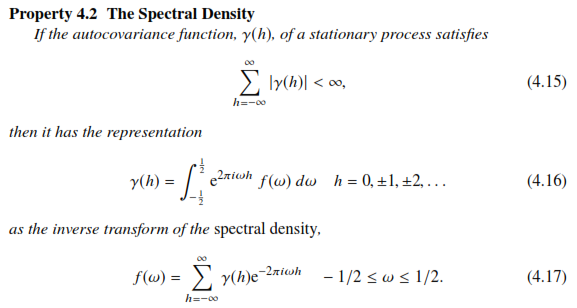
\includegraphics{figure/spec_density} \end{center}

\hl{\textbf{ANS.}} 
\begin{align*}
\lambda(\omega) 
	&=\sum_{h=-\infty}^{\infty}\gamma_h e^{-i\omega h}\\
	&=\sum_{h=-\infty}^{\infty}\frac{\sigma^2 \rho ^{|h|}}{1-\rho^2}e^{-i\omega h}\\
	&=\frac{\sigma^2}{1-\rho^2} + \underbrace{\sum_{h=1}^{\infty}\frac{\sigma^2}{1-\rho^2}\rho^h\left[e^{-i\omega h} + e^{i\omega h}\right]}_{\text{use geometric sum formula}}\\
	&=\frac{\sigma^2}{1-\rho^2}\left[1 + \sum_{h=1}^{\infty}\left(\rho e^{-i\omega}\right)^h + \sum_{h=1}^{\infty}\left(\rho e^{i\omega}\right)^h\right]	
\end{align*}

\begin{center}\rule{0.5\linewidth}{\linethickness}\end{center}

\begin{center}\rule{0.5\linewidth}{\linethickness}\end{center}

\subsubsection{Question: compute the spectrum of the MA(q) moving
mean,}\label{question-compute-the-spectrum-of-the-maq-moving-mean}

\[ Y_n = \frac{1}{q+1} \sum_{k=0}^q \epsilon_{n-k}.\]

\begin{center}\rule{0.5\linewidth}{\linethickness}\end{center}

\begin{center}\rule{0.5\linewidth}{\linethickness}\end{center}

\subsubsection{Review question: how would you demonstrate the
correctness of the
identity,}\label{review-question-how-would-you-demonstrate-the-correctness-of-the-identity}

\[ e^{i\omega} = \cos(\omega)+i\,\sin(\omega).\]

\todo[inline]{Use Taylor series expansion}

\begin{center}\rule{0.5\linewidth}{\linethickness}\end{center}

\begin{center}\rule{0.5\linewidth}{\linethickness}\end{center}

\subsection{Some data analysis using the frequency
domain}\label{some-data-analysis-using-the-frequency-domain}

\subsubsection{Michigan winters
revisited}\label{michigan-winters-revisited}

\begin{itemize}
\tightlist
\item
  Recall the Ann Arbor January weather data,
\end{itemize}

\begin{Shaded}
\begin{Highlighting}[]
\KeywordTok{system}\NormalTok{(}\StringTok{"head ann_arbor_weather.csv"}\NormalTok{,}\DataTypeTok{intern=}\OtherTok{TRUE}\NormalTok{)}
\end{Highlighting}
\end{Shaded}

\begin{verbatim}
##  [1] "## https://weather-warehouse.com/WeatherHistory/PastWeatherData_AnnArborUnivOfMi_AnnArbor_MI_January.html"
##  [2] "## accessed by ELI on Nov 2, 2015"                                                                        
##  [3] "##"                                                                                                       
##  [4] "## Full column descriptions:"                                                                             
##  [5] "## Lowest Temperature (F)"                                                                                
##  [6] "## Highest Temperature (F)"                                                                               
##  [7] "## Warmest Minimum Temperature (F)"                                                                       
##  [8] "## Coldest Maximum Temperature (F)"                                                                       
##  [9] "## Average Minimum Temperature (F)"                                                                       
## [10] "## Average Maximum Temperature (F)"
\end{verbatim}

\begin{Shaded}
\begin{Highlighting}[]
\NormalTok{y <-}\StringTok{ }\KeywordTok{read.table}\NormalTok{(}\DataTypeTok{file=}\StringTok{"ann_arbor_weather.csv"}\NormalTok{,}\DataTypeTok{header=}\OtherTok{TRUE}\NormalTok{)}
\KeywordTok{head}\NormalTok{(y)}
\end{Highlighting}
\end{Shaded}

\begin{verbatim}
##   Year Low High Hi_min Lo_max Avg_min Avg_max Mean Precip Snow Hi_Pricip
## 1 1900  -7   50     36     12    18.0    34.7 26.3   1.06  4.0      0.28
## 2 1901  -7   48     37     20    17.0    31.8 24.4   1.45 10.1      0.40
## 3 1902  -4   41     27     11    15.0    30.4 22.7   0.60  6.0      0.25
## 4 1903  -7   50     36     12    15.1    29.6 22.4   1.27  7.3      0.40
## 5 1904 -11   38     31      6     8.2    22.9 15.3   2.51 11.0      0.67
## 6 1905  -3   47     32     14    10.9    25.9 18.4   1.64  7.9      0.84
##   Hi_Snow
## 1     1.1
## 2     3.2
## 3     2.5
## 4     3.2
## 5     2.1
## 6     2.5
\end{verbatim}

\begin{Shaded}
\begin{Highlighting}[]
\NormalTok{low <-}\StringTok{ }\NormalTok{y}\OperatorTok{\$}\NormalTok{Low}
\end{Highlighting}
\end{Shaded}

\begin{itemize}
\item
  We have to deal with the NA measurement for 1955. A simple approach is
  to replace the NA by the mean.

  \begin{itemize}
  \item
    What other approaches can you think of for dealing with this missing
    observation?
    \todo[inline]{Can fit it with a suitable mean, can remove it.}
  \item
    What are the strengths and weaknesses of these approaches?
  \end{itemize}
\end{itemize}

\begin{Shaded}
\begin{Highlighting}[]
\NormalTok{low[}\KeywordTok{is.na}\NormalTok{(low)] <-}\StringTok{ }\KeywordTok{mean}\NormalTok{(low, }\DataTypeTok{na.rm=}\OtherTok{TRUE}\NormalTok{)}
\end{Highlighting}
\end{Shaded}

\begin{Shaded}
\begin{Highlighting}[]
\KeywordTok{spectrum}\NormalTok{(low, }\DataTypeTok{main=}\StringTok{"Unsmoothed periodogram"}\NormalTok{)}
\end{Highlighting}
\end{Shaded}

\begin{center}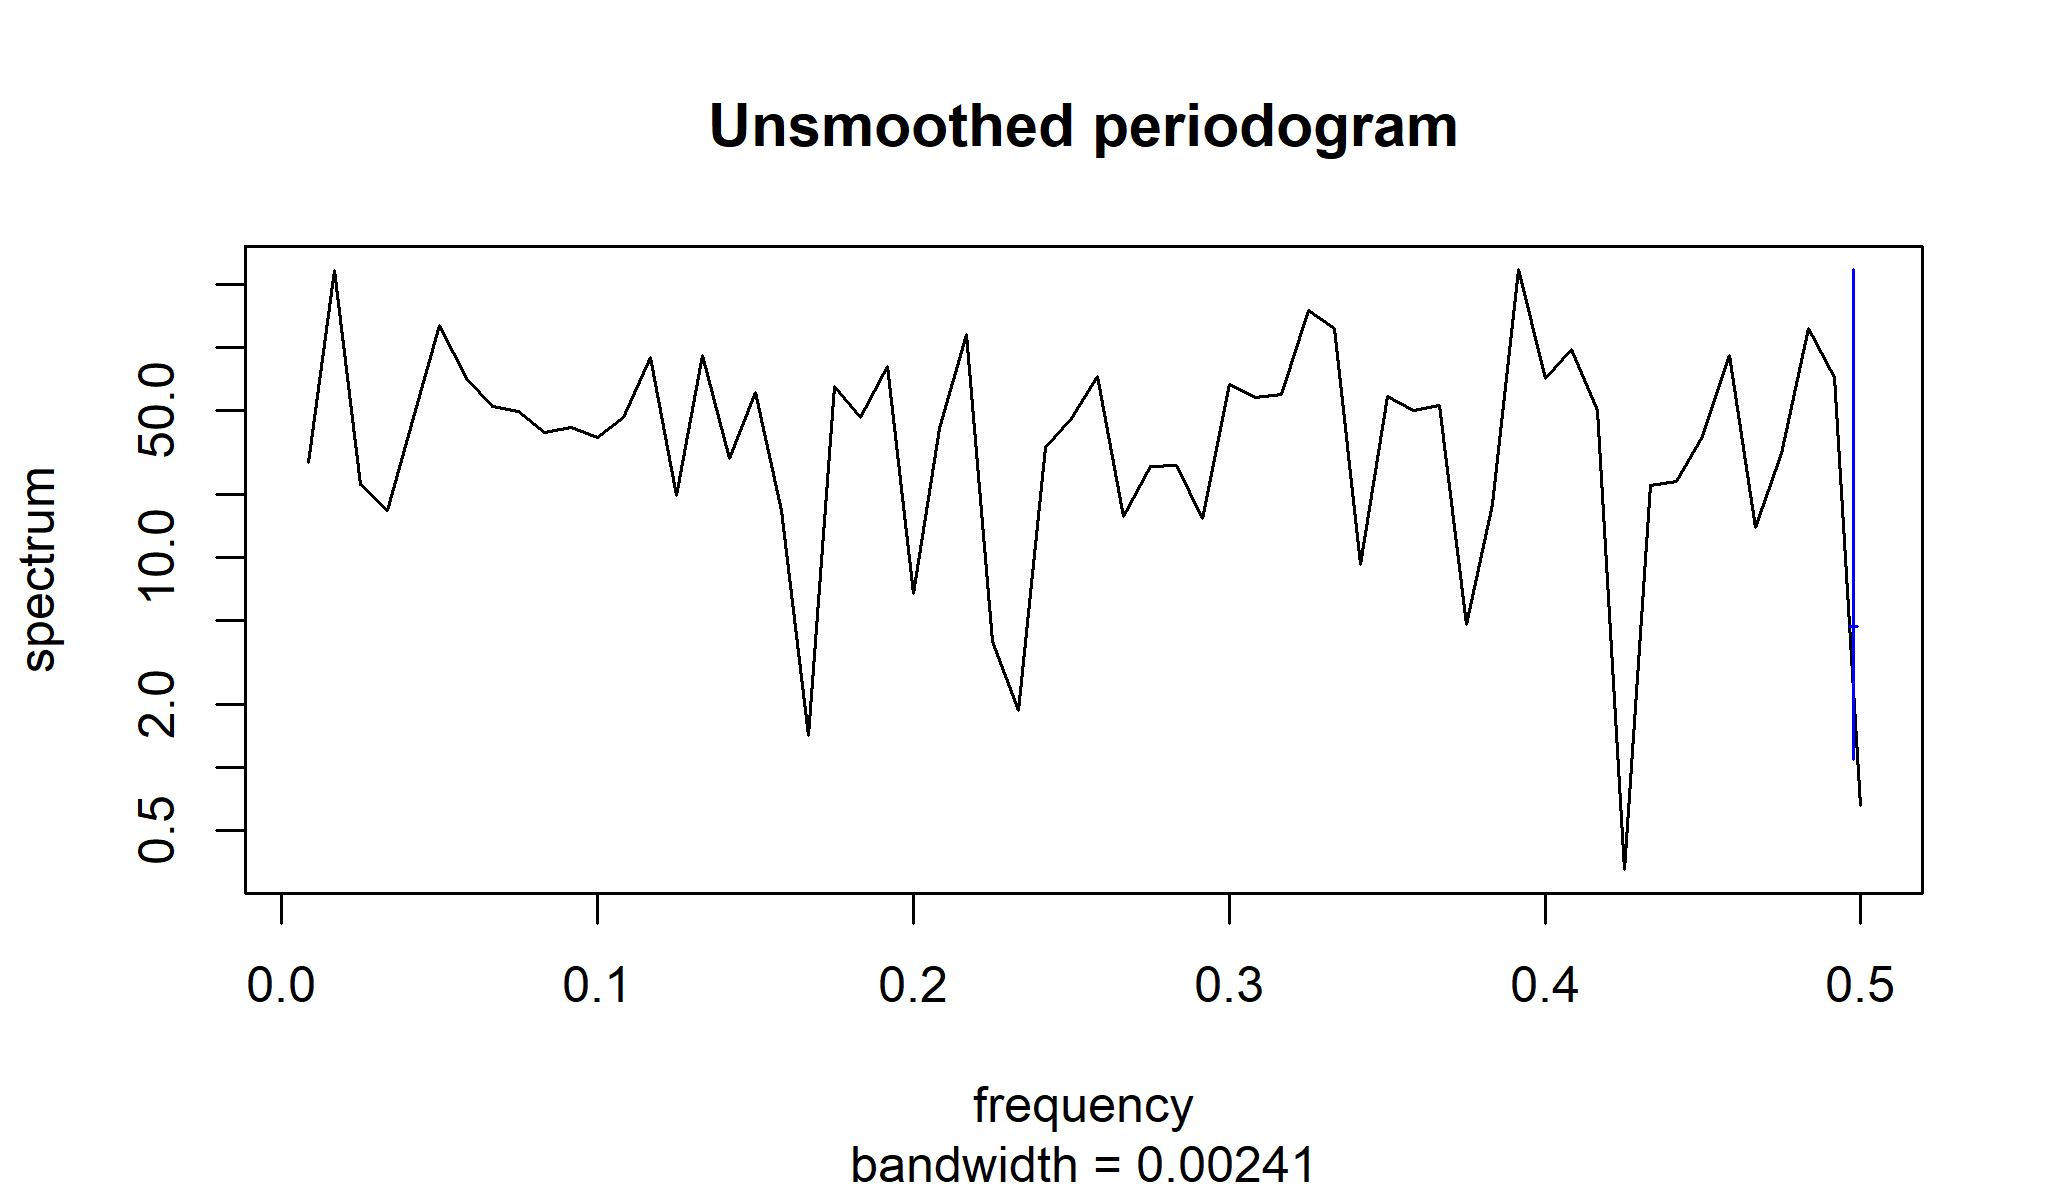
\includegraphics{figure/intro-periodogram-1} \end{center}

\todo[inline]{Here, ``frequency'' is $\omega_{n} = 2\pi n/N$, for $0<n<N/2$. Frequency in ``cycles per data point''}

\begin{itemize}
\tightlist
\item
  To smooth, we use the default periodogram smoother in R
\end{itemize}

\begin{center}\rule{0.5\linewidth}{\linethickness}\end{center}

\begin{center}\rule{0.5\linewidth}{\linethickness}\end{center}

\subsubsection{Question: how does R
smooth?}\label{question-how-does-r-smooth}

\begin{itemize}
\item
  What is the default periodogram smoother in R?
\item
  How should we use it?
\item
  Why is that default chosen?
\end{itemize}

\begin{center}\rule{0.5\linewidth}{\linethickness}\end{center}

\begin{center}\rule{0.5\linewidth}{\linethickness}\end{center}

\begin{Shaded}
\begin{Highlighting}[]
\KeywordTok{spectrum}\NormalTok{(low,}\DataTypeTok{spans=}\KeywordTok{c}\NormalTok{(}\DecValTok{3}\NormalTok{,}\DecValTok{5}\NormalTok{,}\DecValTok{3}\NormalTok{), }\DataTypeTok{main=}\StringTok{"Smoothed periodogram"}\NormalTok{,}\DataTypeTok{ylim=}\KeywordTok{c}\NormalTok{(}\DecValTok{15}\NormalTok{,}\DecValTok{100}\NormalTok{))}
\end{Highlighting}
\end{Shaded}

\begin{center}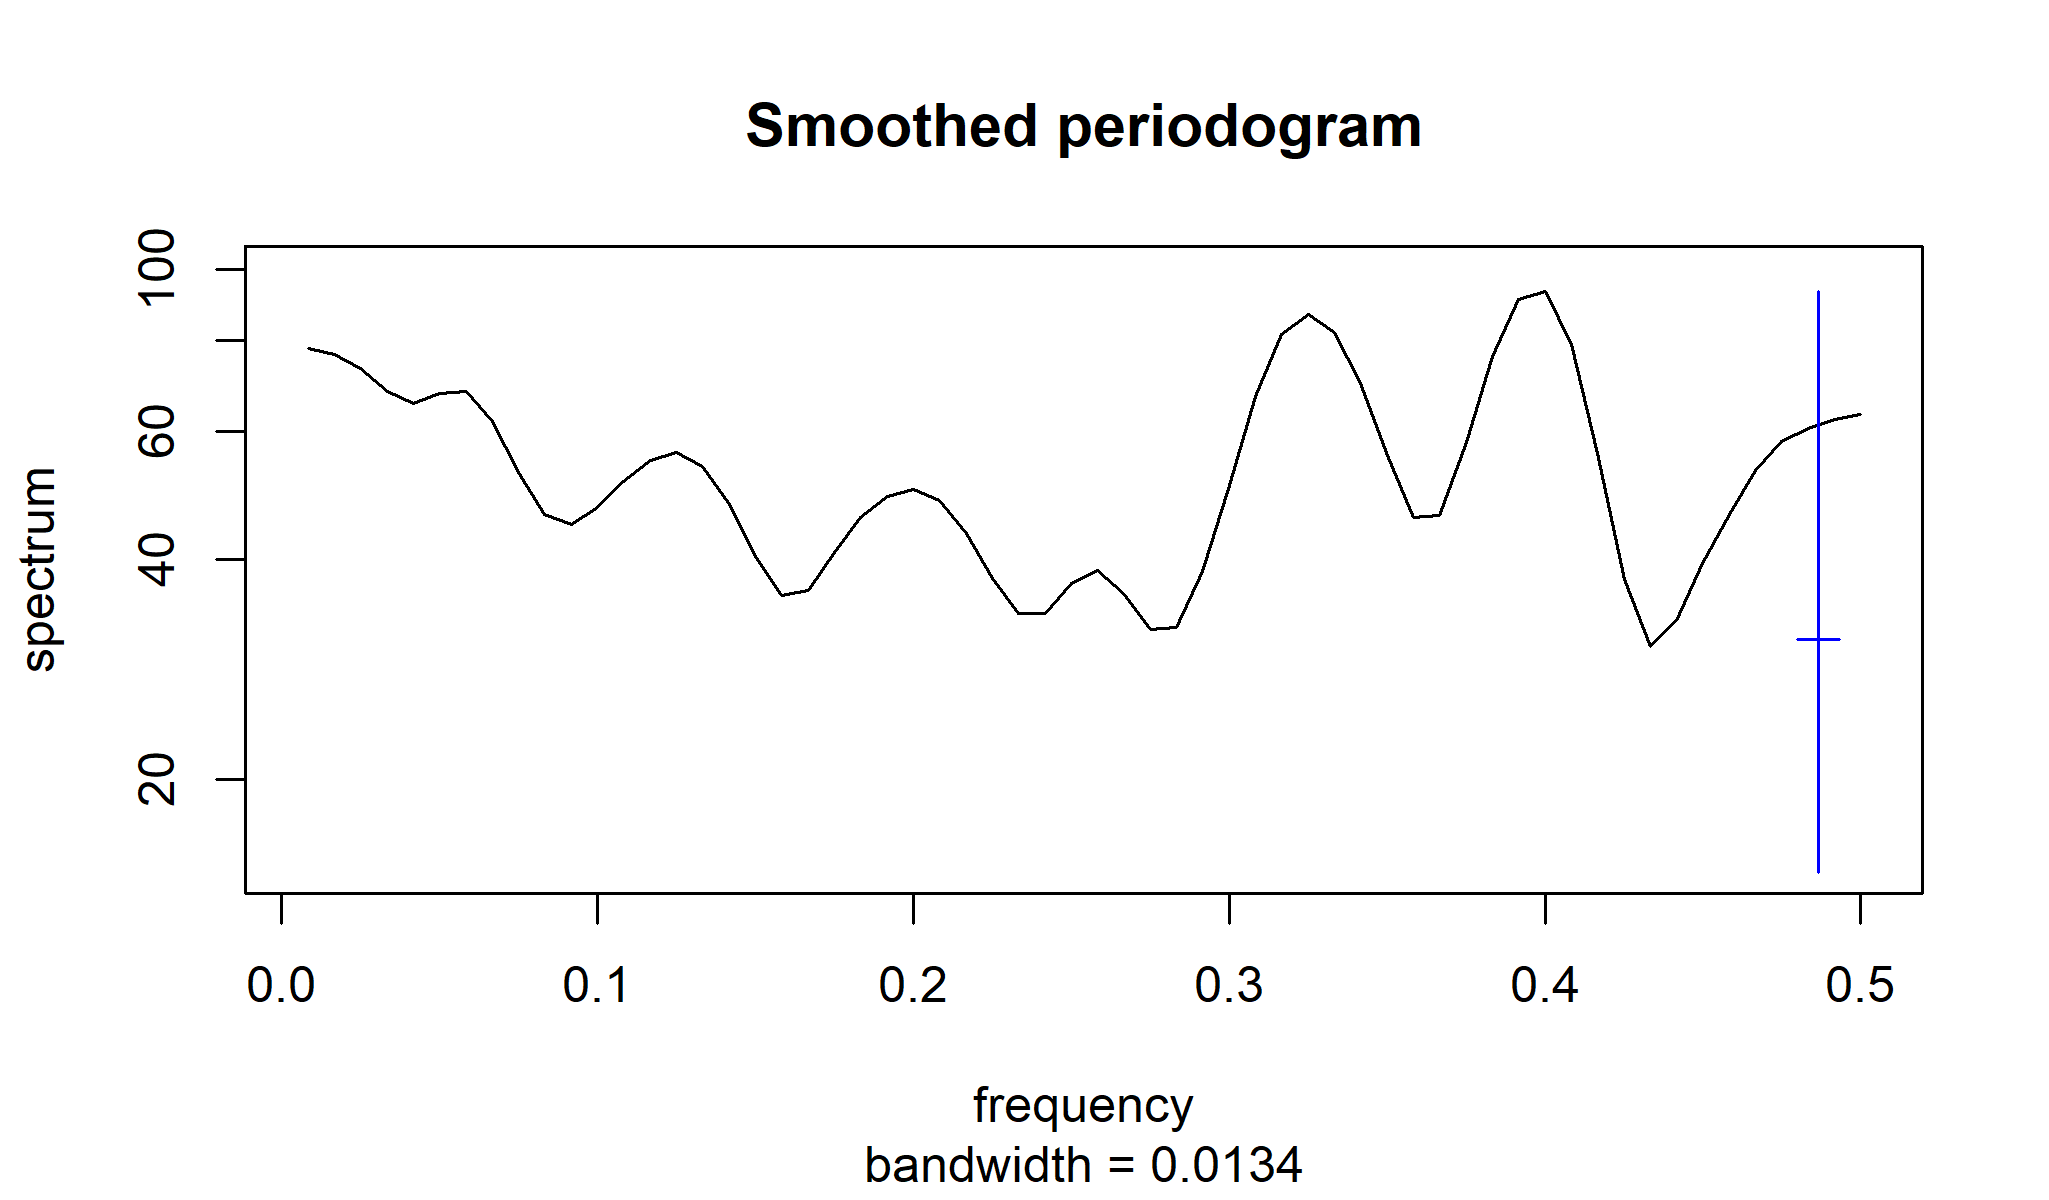
\includegraphics{figure/intro-smoothed_periodogram-1} \end{center}

\begin{center}\rule{0.5\linewidth}{\linethickness}\end{center}

\begin{center}\rule{0.5\linewidth}{\linethickness}\end{center}

\subsubsection{More details on computing and smoothing the
periodogram}\label{more-details-on-computing-and-smoothing-the-periodogram}

\begin{itemize}
\item
  To see what R actually does to compute and smooth the periodogram,
  type \texttt{?spectrum}.
\item
  This will lead you to type \texttt{?spec.pgram}.
\item
  You will see that, by default, \hl{R removes a linear trend, fitted by
  least squares. This may often be a sensible thing to do. Why?}
  
\item
  You will see that R then multiplies the data by a quantity called a
  \href{https://en.wikipedia.org/wiki/Window_function}{\textbf{taper}},
  computed by \texttt{spec.taper}.
\item
  The taper smooths the ends of the time series and removes
  high-frequency artifacts arising from an abrupt start and end to the
  time series.
\item
  Formally, from the perspective of the Fourier transform, the time
  series takes the value zero outside the observed time points \(1:N\).
  The sudden jump to and from zero at the start and end produces
  unwanted effects in the frequency domain.
\item
  The default taper in R smooths the first and last \(p=0.1\) fraction
  of the time points, by modifying the detrended data \(\data{y_{1:N}}\)
  to tapered version \(\data{z_{1:N}}\) defined by
  \[ \data{z_n} = \left\{
  \begin{array}{ll}
  \data{y_n} \big(1-\cos(\pi n/Np)\big)/2 & \mbox{ if $1\le n< Np$ }
  \\
  \data{y_n}  & \mbox{ if $Np \le n \le N(1-p)$ }
  \\
  \data{y_n} \big(1-\cos(\pi [N+1-n]/Np)\big)/2 & \mbox{ if $N(1-p)<n\le N$ }
  \end{array}\right.
  \]
\end{itemize}

\begin{Shaded}
\begin{Highlighting}[]
\KeywordTok{plot}\NormalTok{(}\KeywordTok{spec.taper}\NormalTok{(}\KeywordTok{rep}\NormalTok{(}\DecValTok{1}\NormalTok{,}\DecValTok{100}\NormalTok{)),}\DataTypeTok{type=}\StringTok{"l"}\NormalTok{,}
  \DataTypeTok{main=}\StringTok{"Default taper in R for a time series of length 100"}\NormalTok{)}
\KeywordTok{abline}\NormalTok{(}\DataTypeTok{v=}\KeywordTok{c}\NormalTok{(}\DecValTok{10}\NormalTok{,}\DecValTok{90}\NormalTok{),}\DataTypeTok{lty=}\StringTok{"dotted"}\NormalTok{,}\DataTypeTok{col=}\StringTok{"red"}\NormalTok{)}
\end{Highlighting}
\end{Shaded}

\begin{center}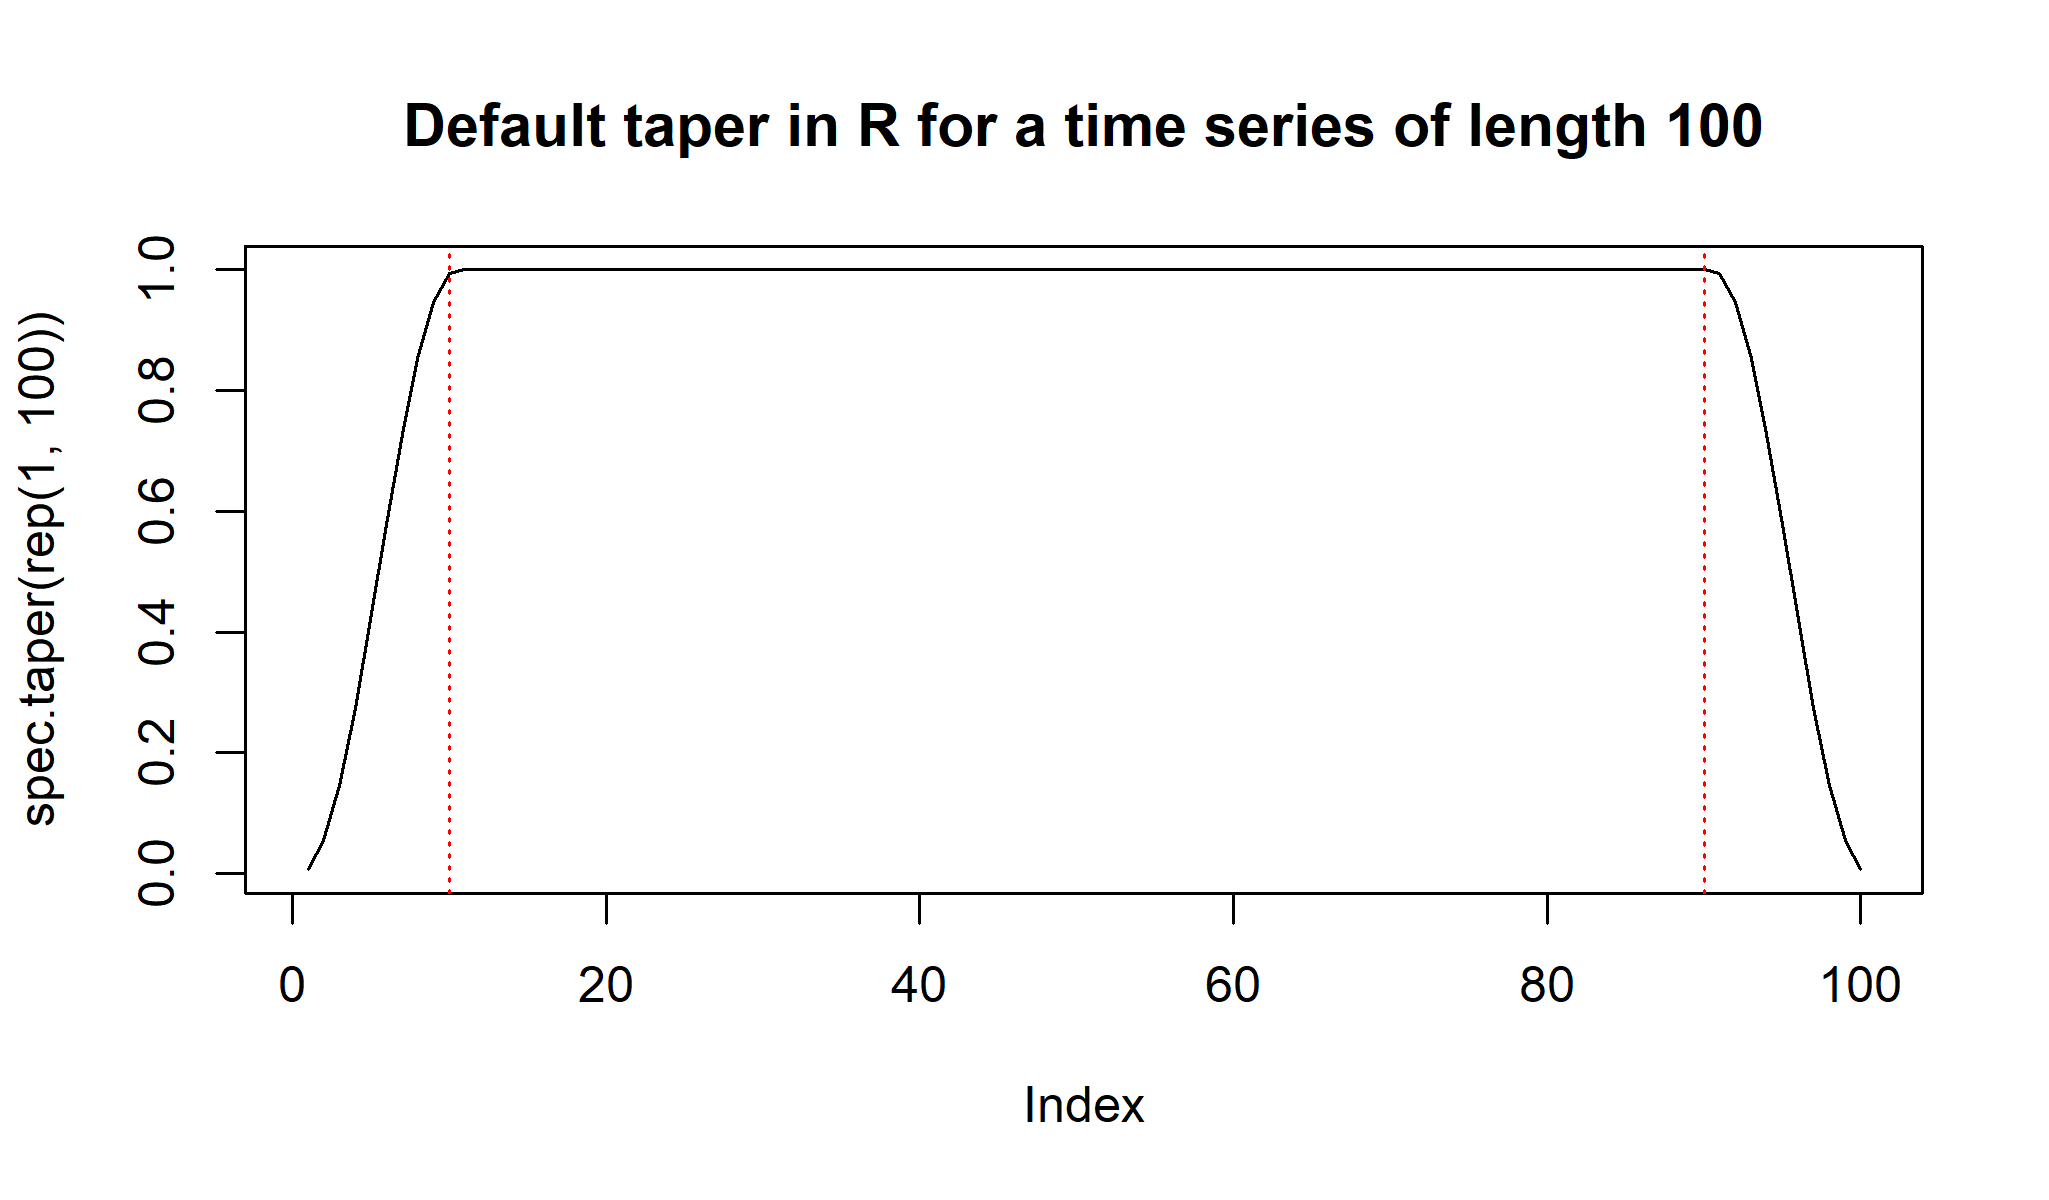
\includegraphics{figure/intro-taper_plot-1} \end{center}

\begin{center}\rule{0.5\linewidth}{\linethickness}\end{center}

\begin{center}\rule{0.5\linewidth}{\linethickness}\end{center}

\subsubsection{Spectral density estimation by fitting a
model}\label{spectral-density-estimation-by-fitting-a-model}

\begin{itemize}
\tightlist
\item
  Another standard way to estimate the spectrum is to fit an AR(p) model
  with \(p\) selected by AIC.
\end{itemize}

\begin{Shaded}
\begin{Highlighting}[]
\KeywordTok{spectrum}\NormalTok{(low,}\DataTypeTok{method=}\StringTok{"ar"}\NormalTok{, }\DataTypeTok{main=}\StringTok{"Spectrum estimated via AR model picked by AIC"}\NormalTok{)}
\end{Highlighting}
\end{Shaded}

\begin{center}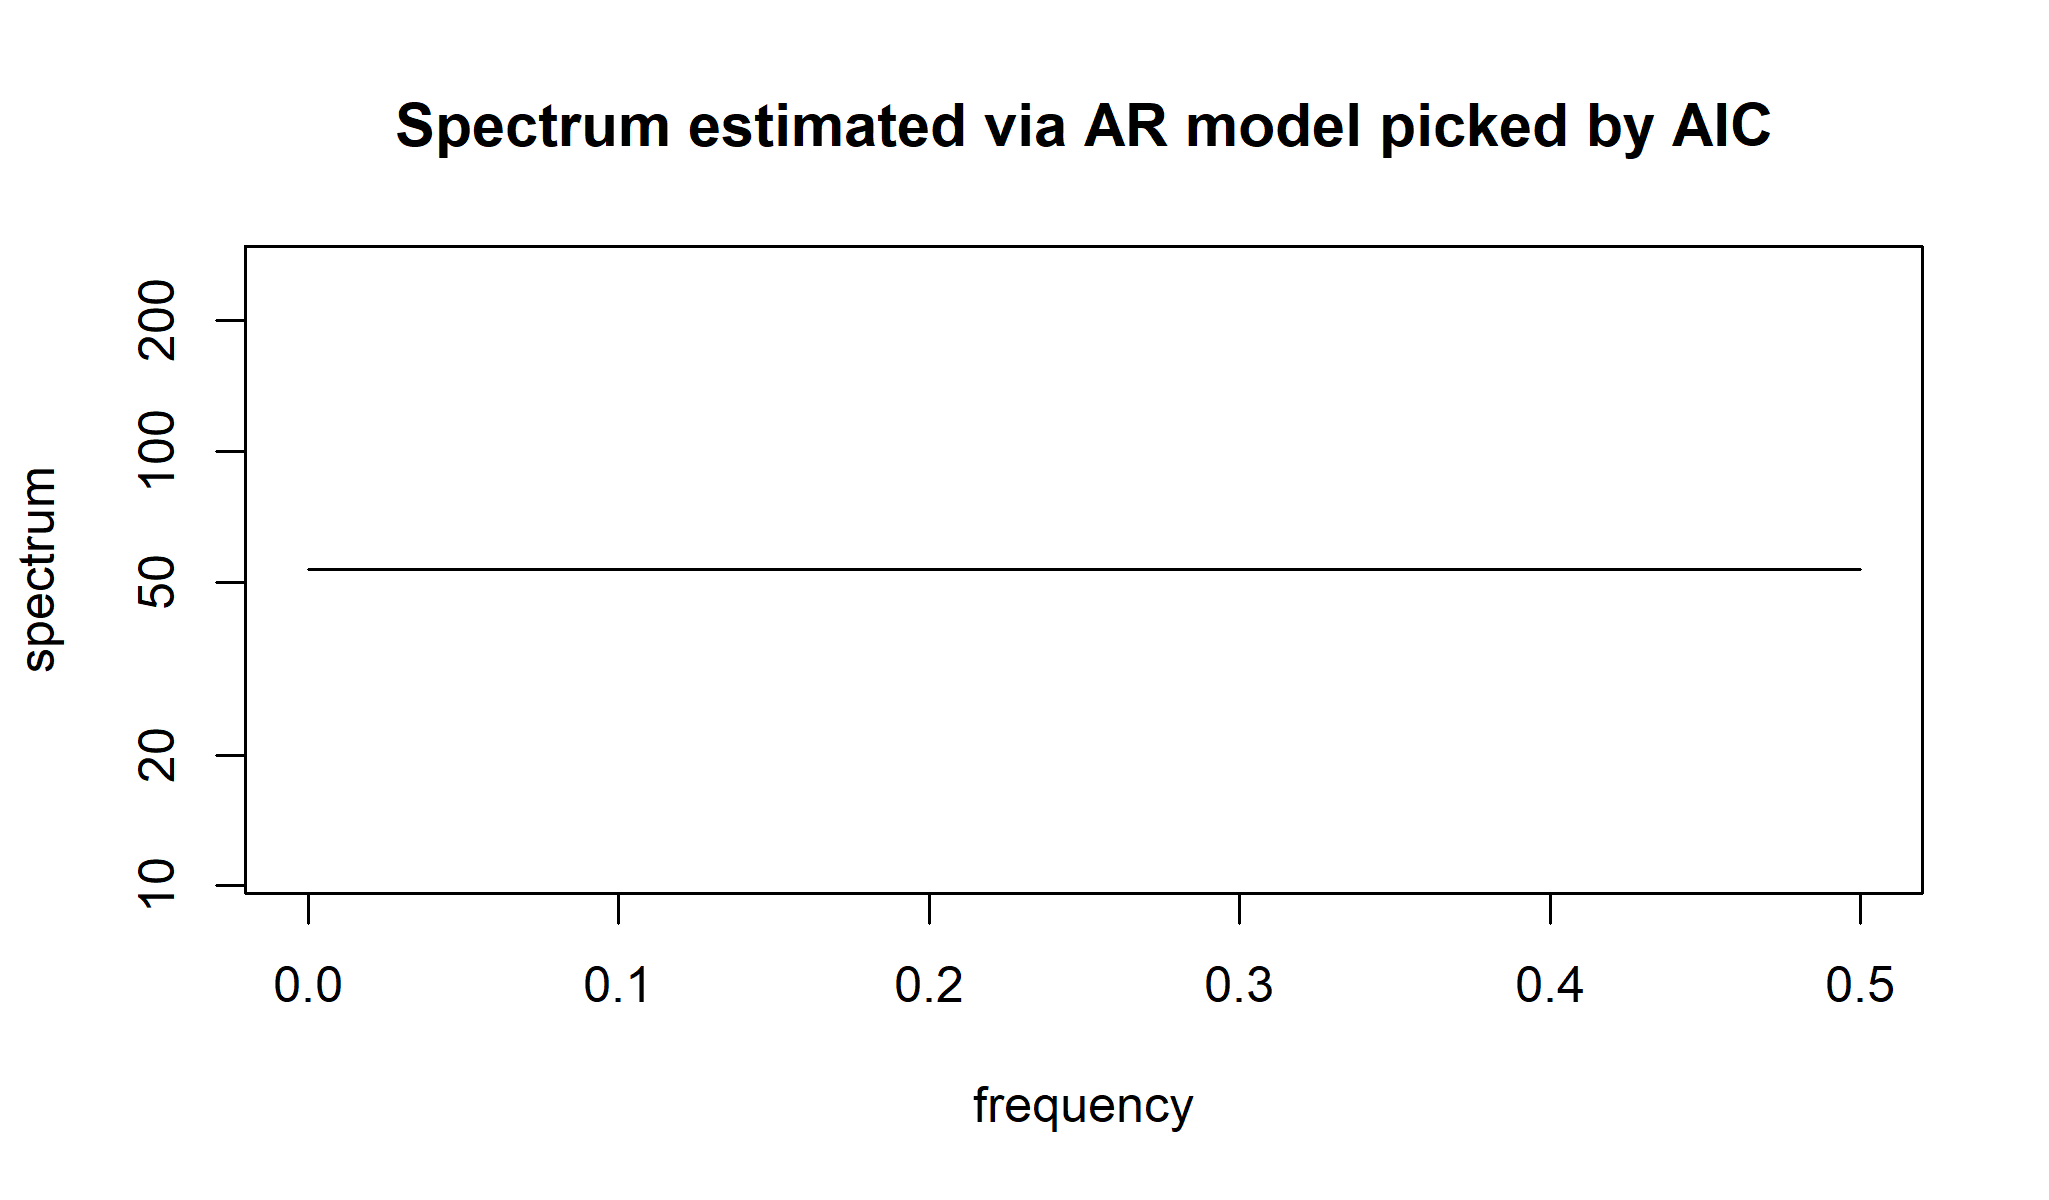
\includegraphics{figure/intro-ar_periodogram-1} \end{center}

\begin{center}\rule{0.5\linewidth}{\linethickness}\end{center}

\begin{center}\rule{0.5\linewidth}{\linethickness}\end{center}

\subsubsection{Fitting a signal plus white noise
model}\label{fitting-a-signal-plus-white-noise-model}

\begin{itemize}
\item
  Since this time series is well modeled by white noise, we could fit a
  signal plus white noise model. This might be a more sensitive way to
  look for a trend.
\item
  Let's try some low-order polynomial trend specifications.
\end{itemize}

\begin{Shaded}
\begin{Highlighting}[]
\NormalTok{lm0 <-}\StringTok{ }\KeywordTok{lm}\NormalTok{(Low}\OperatorTok{~}\DecValTok{1}\NormalTok{,}\DataTypeTok{data=}\NormalTok{y)}
\NormalTok{lm1 <-}\StringTok{ }\KeywordTok{lm}\NormalTok{(Low}\OperatorTok{~}\NormalTok{Year,}\DataTypeTok{data=}\NormalTok{y)}
\NormalTok{lm2 <-}\StringTok{ }\KeywordTok{lm}\NormalTok{(Low}\OperatorTok{~}\NormalTok{Year}\OperatorTok{+}\KeywordTok{I}\NormalTok{(Year}\OperatorTok{^}\DecValTok{2}\NormalTok{),}\DataTypeTok{data=}\NormalTok{y)}
\NormalTok{lm3 <-}\StringTok{ }\KeywordTok{lm}\NormalTok{(Low}\OperatorTok{~}\NormalTok{Year}\OperatorTok{+}\KeywordTok{I}\NormalTok{(Year}\OperatorTok{^}\DecValTok{2}\NormalTok{)}\OperatorTok{+}\KeywordTok{I}\NormalTok{(Year}\OperatorTok{^}\DecValTok{3}\NormalTok{),}\DataTypeTok{data=}\NormalTok{y)}
\NormalTok{poly_aic <-}\StringTok{ }\KeywordTok{matrix}\NormalTok{( }\KeywordTok{c}\NormalTok{(}\KeywordTok{AIC}\NormalTok{(lm0),}\KeywordTok{AIC}\NormalTok{(lm1),}\KeywordTok{AIC}\NormalTok{(lm2),}\KeywordTok{AIC}\NormalTok{(lm3)), }\DataTypeTok{nrow=}\DecValTok{1}\NormalTok{,}
   \DataTypeTok{dimnames=}\KeywordTok{list}\NormalTok{(}\StringTok{"<b>AIC</b>"}\NormalTok{, }\KeywordTok{paste}\NormalTok{(}\StringTok{"order"}\NormalTok{,}\DecValTok{0}\OperatorTok{:}\DecValTok{3}\NormalTok{)))}
\KeywordTok{require}\NormalTok{(knitr)}
\KeywordTok{kable}\NormalTok{(poly_aic,}\DataTypeTok{digits=}\DecValTok{1}\NormalTok{)}
\end{Highlighting}
\end{Shaded}

\begin{longtable}[]{@{}lrrrr@{}}
\toprule
& order 0 & order 1 & order 2 & order 3\tabularnewline
\midrule
\endhead
AIC & 780.9 & 781.6 & 783.6 & 783.8\tabularnewline
\bottomrule
\end{longtable}

\begin{itemize}
\item
  Still no evidence suggesting anything other than a white noise model.
\item
  Now, let's remind ourselves what the data look like.
\end{itemize}

\begin{Shaded}
\begin{Highlighting}[]
\KeywordTok{plot}\NormalTok{(Low}\OperatorTok{~}\NormalTok{Year,}\DataTypeTok{data=}\NormalTok{y,}\DataTypeTok{type=}\StringTok{"l"}\NormalTok{)}
\end{Highlighting}
\end{Shaded}

\begin{center}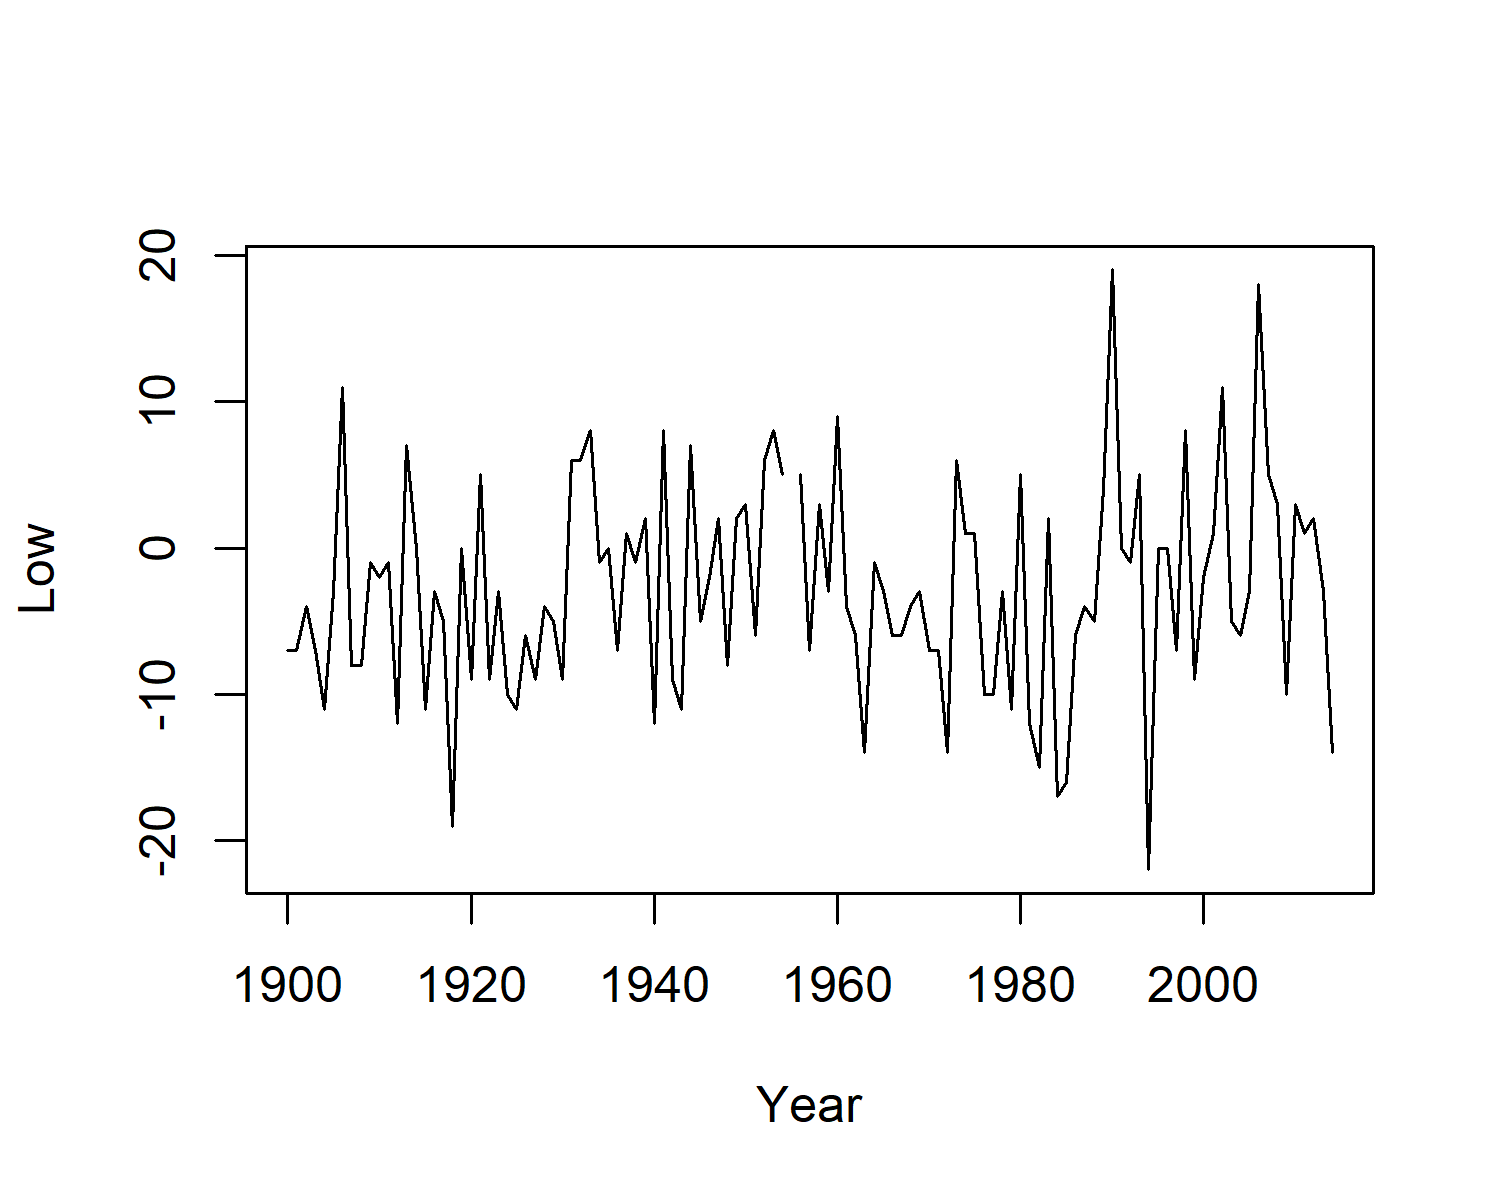
\includegraphics{figure/intro-plot_jan_temp-1} \end{center}

\begin{itemize}
\item
  Our eye may see a trend, and recall that it looks a bit like the
  global temperature trend.
\item
  Let's try fitting global temperature as an explanatory variable.
\end{itemize}

\begin{Shaded}
\begin{Highlighting}[]
\NormalTok{Z <-}\StringTok{ }\KeywordTok{read.table}\NormalTok{(}\StringTok{"Global_Temperature.txt"}\NormalTok{,}\DataTypeTok{header=}\OtherTok{TRUE}\NormalTok{)}
\NormalTok{global_temp <-}\StringTok{ }\NormalTok{Z}\OperatorTok{\$}\NormalTok{Annual[Z}\OperatorTok{\$}\NormalTok{Year }\OperatorTok{\%in\%}\StringTok{ }\NormalTok{y}\OperatorTok{\$}\NormalTok{Year]}
\NormalTok{lm_global <-}\StringTok{ }\KeywordTok{lm}\NormalTok{(Low}\OperatorTok{~}\NormalTok{global_temp,}\DataTypeTok{data=}\NormalTok{y)}
\KeywordTok{AIC}\NormalTok{(lm_global)}
\end{Highlighting}
\end{Shaded}

\begin{verbatim}
## [1] 779.8877
\end{verbatim}

\begin{itemize}
\tightlist
\item
  Got it! We have an explantion of the trend that makes scientific
  sense. However, the model is prefered by AIC but is \hl{not quite
  statistically significant viewed as a 2-sided test against a null of
  white noise via a t-statistic for the estimated coefficient}:
\end{itemize}

\begin{Shaded}
\begin{Highlighting}[]
\KeywordTok{summary}\NormalTok{(lm_global)}
\end{Highlighting}
\end{Shaded}

\begin{verbatim}
## 
## Call:
## lm(formula = Low ~ global_temp, data = y)
## 
## Residuals:
##      Min       1Q   Median       3Q      Max 
## -20.1554  -4.5079  -0.1595   4.1068  20.3959 
## 
## Coefficients:
##             Estimate Std. Error t value Pr(>|t|)    
## (Intercept)  -3.0413     0.6916  -4.397 2.51e-05 ***
## global_temp   3.7396     2.1530   1.737   0.0851 .  
## ---
## Signif. codes:  0 '***' 0.001 '**' 0.01 '*' 0.05 '.' 0.1 ' ' 1
## 
## Residual standard error: 7.273 on 112 degrees of freedom
##   (1 observation deleted due to missingness)
## Multiple R-squared:  0.02623,    Adjusted R-squared:  0.01754 
## F-statistic: 3.017 on 1 and 112 DF,  p-value: 0.08515
\end{verbatim}

\todo[inline]{1-sided p-value is $0.043 < 0.05$, 2--sided p-value is 0.085}

\begin{center}\rule{0.5\linewidth}{\linethickness}\end{center}

\begin{center}\rule{0.5\linewidth}{\linethickness}\end{center}

\subsubsection{Question: is a 2-sided test or a 1-sided test more
reasonable
here?}\label{question-is-a-2-sided-test-or-a-1-sided-test-more-reasonable-here}

\begin{itemize}
\tightlist
\item
  What is the p-value for the 1-sided test?
\end{itemize}

\begin{center}\rule{0.5\linewidth}{\linethickness}\end{center}

\begin{center}\rule{0.5\linewidth}{\linethickness}\end{center}

\begin{itemize}
\item
  Perhaps we now have a satisfactory understanding of Ann Arbor January
  low temperatures: random, white noise, variation around the global
  mean temperature trend.
\item
  With noisy data, uncovering what is going on can take careful data
  analysis together with scientific reasoning.
\item
  What could we do to improve the signal to noise ratio in this
  analysis?
\end{itemize}

\begin{center}\rule{0.5\linewidth}{\linethickness}\end{center}

\begin{center}\rule{0.5\linewidth}{\linethickness}\end{center}

\subsubsection{Question: Why might you expect the estimated coefficient
to be statistically insignificant in this analysis, even if the model
with global mean temperature plus trend is
correct?}\label{question-why-might-you-expect-the-estimated-coefficient-to-be-statistically-insignificant-in-this-analysis-even-if-the-model-with-global-mean-temperature-plus-trend-is-correct}

Hint: notice the standard error on the coefficient, together with
consideration of possible values of the coefficient in a scientifically
plausible model.



\begin{center}\rule{0.5\linewidth}{\linethickness}\end{center}

\begin{center}\rule{0.5\linewidth}{\linethickness}\end{center}

\subsection{Units of frequency and
period}\label{units-of-frequency-and-period}

\begin{itemize}
\item
  It is always good practice to be explicit about the units of
  quantities. For frequency domain analysis we can consider various
  options for units of frequency.
\item
  For a frequency component corresponding to \(\sin(2\pi\omega n)\) or
  \(\cos(2\pi\omega n)\), we say that the frequency is \(\omega\)
  \textbf{cycles per unit time}.
\item
  Suppose the time series consists of equally spaced observations, with
  \(t_{n}-t_{n-1}=\Delta\) years. Then we say that the frequency is
  \(\omega/\Delta\) \textbf{cycles per year}.
\item
  For a frequency component corresponding to \(\sin(\nu t)\) or
  \(\cos(\nu t)\), we say that the frequency is \(\nu\) \textbf{radians
  per unit time}.
\item
  The \textbf{period} of an oscillation is the time for one cycle. So,
  when frequency is measured in cycles per time, we have
  \[ \mbox{period} = \frac{1}{\mbox{frequency}}.\] Thus, for a frequency
  component corresponding to \(\sin(2\pi\omega n)\) or
  \(\cos(2\pi\omega n)\), the period is \(1/\omega\) observation
  intervals.
\item
  When the observation intervals have constant time length (years,
  seconds, etc) we should use those units for the period.
\end{itemize}

\begin{center}\rule{0.5\linewidth}{\linethickness}\end{center}

\begin{center}\rule{0.5\linewidth}{\linethickness}\end{center}


\end{document}
